\documentclass[handout]{beamer}
\mode<presentation>
{
  \usetheme{Warsaw}
  \definecolor{mcgarnet}{rgb}{0.38, 0, 0.08}
  \definecolor{mcgray}{rgb}{0.6, 0.6, 0.6}
  \setbeamercolor{structure}{fg=mcgarnet,bg=mcgray}
  %\setbeamercovered{transparent}
}


\usepackage[english]{babel}
\usepackage[latin1]{inputenc}
\usepackage{times}
\usepackage[T1]{fontenc}
\usepackage{tikz}
\usepackage{graphicx}
\usepackage{caption}
\usepackage{enumerate}

\newcommand{\imagesource}[1]{{\centering\hfill\break\hbox{\scriptsize Image Source:\thinspace{\small\itshape wikipedia.org}}\par}}

\title{OOPs: The Harsh Realities of Programming}


\author{Robert Lowe\\}

\institute[Maryville College] % (optional, but mostly needed)
{
  Division of Mathematics and Computer Science\\
  Maryville College
}

\date[]{}
\subject{}

\pgfdeclareimage[height=0.5cm]{university-logo}{images/Maryville-College}
\logo{\pgfuseimage{university-logo}}



\AtBeginSection[]
{
  \begin{frame}<beamer>{Outline}
    \tableofcontents[currentsection]
  \end{frame}
}


\begin{document}

\begin{frame}
  \titlepage
\end{frame}

\begin{frame}{Outline}
  \tableofcontents
\end{frame}


% Structuring a talk is a difficult task and the following structure
% may not be suitable. Here are some rules that apply for this
% solution: 

% - Exactly two or three sections (other than the summary).
% - At *most* three subsections per section.
% - Talk about 30s to 2min per frame. So there should be between about
%   15 and 30 frames, all told.

% - A conference audience is likely to know very little of what you
%   are going to talk about. So *simplify*!
% - In a 20min talk, getting the main ideas across is hard
%   enough. Leave out details, even if it means being less precise than
%   you think necessary.
% - If you omit details that are vital to the proof/implementation,
%   just say so once. Everybody will be happy with that.
\section{Course Overview}
\begin{frame}
   \frametitle{Preliminaries}
   \begin{columns}
      \column{0.6\textwidth}
      Required Materials
      \begin{itemize}
         \item Big C++ 2nd Edition by Cay Horstmann
         \item An Account on smc.cs.maryvillecollege.edu
      \end{itemize}
      \begin{block}{Catalog Description}
      A continuation of Computer Science 111 with emphasis on advanced programming features. Laboratory work supplements and expands lecture topics and offers supervised practice using programming.
      \end{block}
      \column{0.4\textwidth}
      
\includegraphics[width=\textwidth]{images/bigcpp}
   \end{columns}
\end{frame}

\begin{frame}
   \frametitle{Recommended Supplementary Text}
   \begin{columns}
      \column{0.6\textwidth}
      {\em The C++ Programming Language} 4th Edition by Bjarne Stroustrup
      \begin{itemize}
         \item Written by the creator of C++
         \item Serves as a Good Reference
         \item Very in-depth Explanations of The Language
         \item This should be on the bookshelf of all serious C++ programmers.
      \end{itemize}
      \column{0.4\textwidth}
      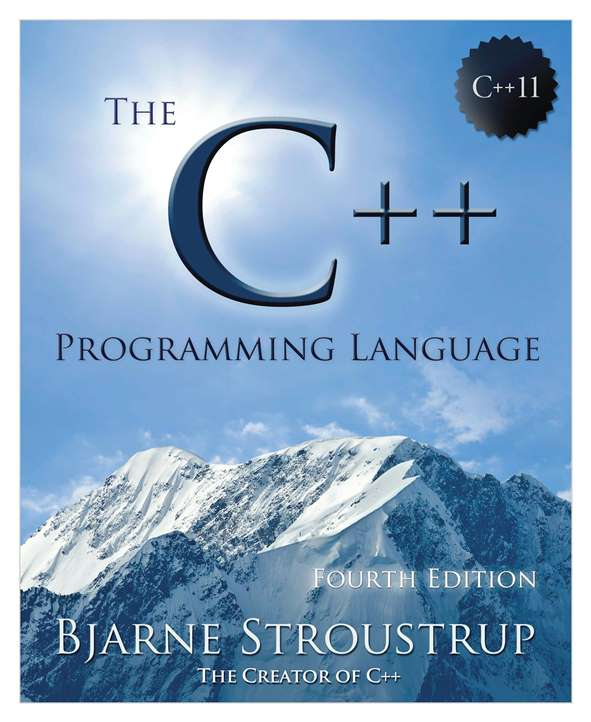
\includegraphics[width=\textwidth]{images/stroustrup}
   \end{columns}
\end{frame}

\begin{frame}
   \frametitle{Course Goals}
   \begin{itemize}
      \item Gain an advanced understanding of Object Oriented Programming.
      \item Learn to use Object Oriented Analysis and Design to build large complex 
            programs. 
      \item Gain a preliminary understanding of low level programming concepts,
            especially memory addressing.
      \item Increase your knowledge of using and programming the UNIX operating       
            system.
      \item Hone your knowledge of programming tools like make, g++, and gdb.
      \item Learn new tools, like git.
   \end{itemize}
\end{frame}

\begin{frame}
    \frametitle{Grading}
    \textbf{Grading}
    
    \begin{tabular}{|l|r|}
       \hline
       Labs & 15\%\\
       \hline
       Programming Assignments & 50\%\\
       \hline
       Exams & 35\%\\
       \hline
    \end{tabular}
\end{frame}

\begin{frame}
   \frametitle{Summary of Classroom Expectations}
   \begin{itemize}
      \item Show up for class.
      \item Don't cheat.
      \item Attempt all the work.
      \item Ask lots of questions.
      \item Late assignments will generally not be accepted.
      \item Don't Panic!
   \end{itemize}
\end{frame}

\begin{frame}
   \frametitle{Outline of Major Topics}
   \begin{enumerate}[I.]
   \item Object Oriented Programming
       \begin{enumerate}[a.]
       \item Classes and Objects
       \item Inheritance and Polymorphism
       \item Overloaded Operators and Functions
       \item Object Oriented Analysis and Design
       \end{enumerate}
   \item Problem Solving Techniques
       \begin{enumerate}[a.]
       \item Recursion
       \item Backtracking
       \end{enumerate}
   \item Tools and Techniques
       \begin{enumerate}[a.]
       \item gdb 
       \item UNIX System API
       \item Exceptions
       \end{enumerate}
   \end{enumerate}
\end{frame}

\section{Complexity and the Nature of Programming}
\begin{frame}
   \frametitle{Software Development Life Cycle}
   \begin{columns}
   \column{0.6\textwidth}
   Programming Is:
   \begin{itemize}
   \item Expensive
   \item Very Complex
   \item Critical
   \end{itemize}
   
   \begin{block}{The Ninety-Ninety Rule}<2->
    The first 90 percent of the code accounts for the first 90 percent of the development time. The remaining 10 percent of the code accounts for the other 90 percent of the development time.
    
    -- Tom Cargill, Bell Labs
   \end{block} 
   
   \column{0.4\textwidth}
   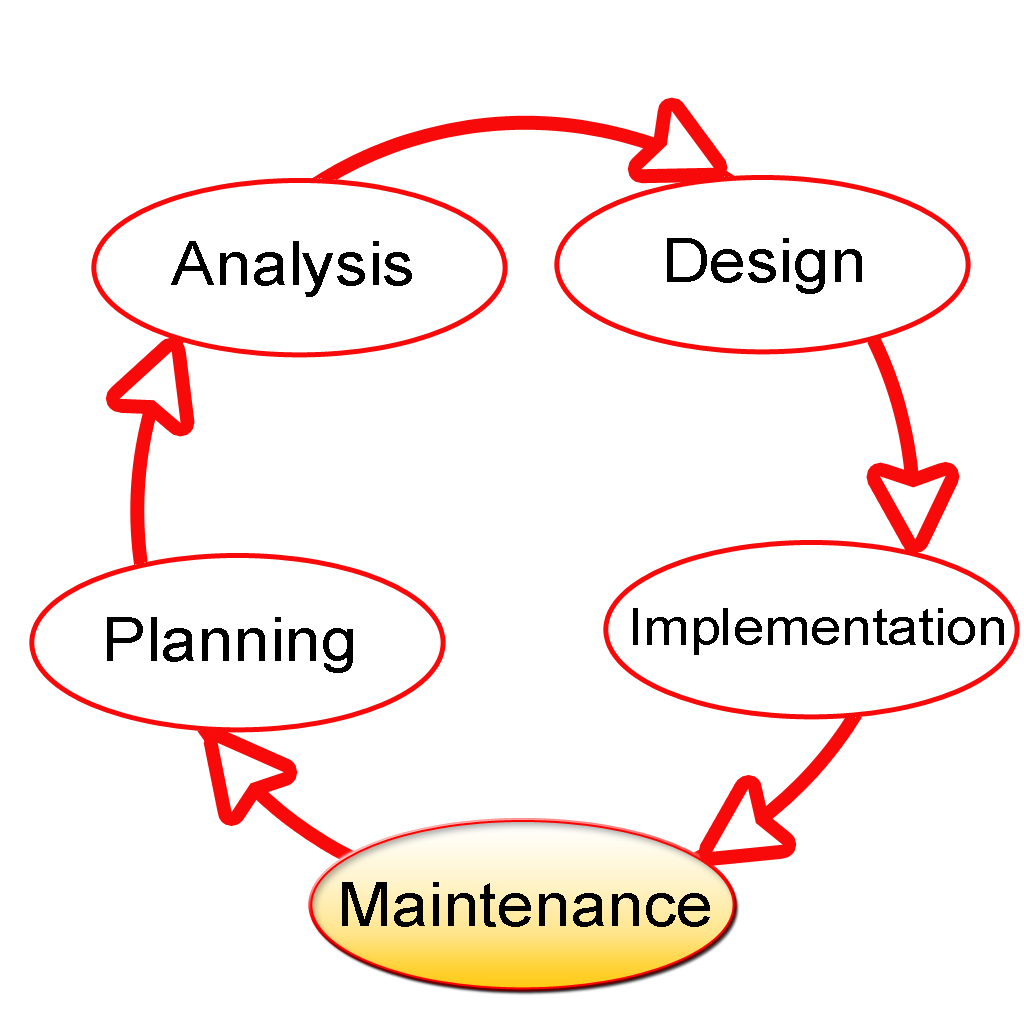
\includegraphics[width=\textwidth]{images/sdlc}
   \imagesource{wikipedia.org}
   \end{columns}
\end{frame}

\begin{frame}
   \frametitle{Coping with Complexity}
   \begin{itemize}
   \item<1-> The Main Challenge is Dealing With Complexity
   \item<2-> Analyze Big Tasks
   \item<3-> Decompose Big Tasks
   \item<4-> Encode Tasks into Computer Code
   \end{itemize}
\end{frame}

\begin{frame}
   \frametitle{Coping with Customers}
   \begin{itemize}
   \item<2-> Real world customers are not very tech savvy.
   \item<3-> Often, programs perform tasks outside of the programmer's expertise.
   \item<4-> Many iterations are needed to capture requirements.
   \item<5-> Even then, requirements are typically vague!
   \end{itemize}
\end{frame}

\begin{frame}
   \frametitle{What Makes Programming Difficult}
   \begin{itemize}
   \item Complexity
   \item Vague and Underdeveloped Requirements
   \item Time Pressure
   \item One-Off Nature of Programs
   \end{itemize}
\end{frame}

\begin{frame}
   \frametitle{Programming Paradigms}
   Programming paradigms represent ways of thinking and methods of
   decomposition.
   \begin{description}
   \item[Imperative Programming] All statements are direct commands
     which alter the program's state.  (ex. Assembly and ALGOL)
   \item[Procedural Programming] Programs are decomposed into sub-routines.
     (ex. C and Pascal )
   \item[Functional Programming] Computation is represented as mathematical
     functions.  (ex. LISP and Erlang)
   \item[Object Oriented Programming] Programs are decomposed into objects.
     (ex. C++ and C\#)
   \end{description}
\end{frame}

\begin{frame}
   \frametitle{Effective Use of a Programming Language}
   General Tips for Programming Language Use
   \begin{itemize}
   \item<2-> A programming language is a formal representation of ideas.
   \item<3-> Think first and then code!
   \item<4-> Use a language that is well suited to the task at hand.
   \item<5-> Learn the idioms of your language.
   \item<6-> Always use the language to express, rather than obscure, 
       your intentions!
   \end{itemize}
\end{frame}

\section{Overview of Object Oriented Programming}

\begin{frame}
   \frametitle{Objects and Classes}
   \begin{description}
   \item[Object] An entity with state and behavior. (Instance of Classes)
     \begin{itemize}
     \item<2-> Variables
     \item<2-> Concrete Objects
     \end{itemize}
   \item[Class] A collection of objects with identical attributes and
     behaviors.  (Definition of Objects)
     \begin{itemize}
     \item<3-> Member Functions
     \item<3-> Member Variables
     \item<3-> Abstract Entity
   \end{itemize}
   \end{description}
\end{frame}

\begin{frame}
   \frametitle{Parts of Speech and OOP}
   \begin{description}
   \item[Nouns]<2-> Objects and Classes
   \item[Verbs]<3-> Member Functions
   \item[Adjectives]<4-> Member Variables
   \end{description}
\end{frame}

\begin{frame}
   \frametitle{An OOP Translation Example}
   \begin{columns}
   \column{0.5\textwidth}
   \begin{enumerate}
   \item Write some sentences describing the robot and its state.
   \item Write some sentences describing what the robot can do.
   \item Sketch out what a robot class may look like.
   \end{enumerate}
   
   \column{0.4\textwidth}
   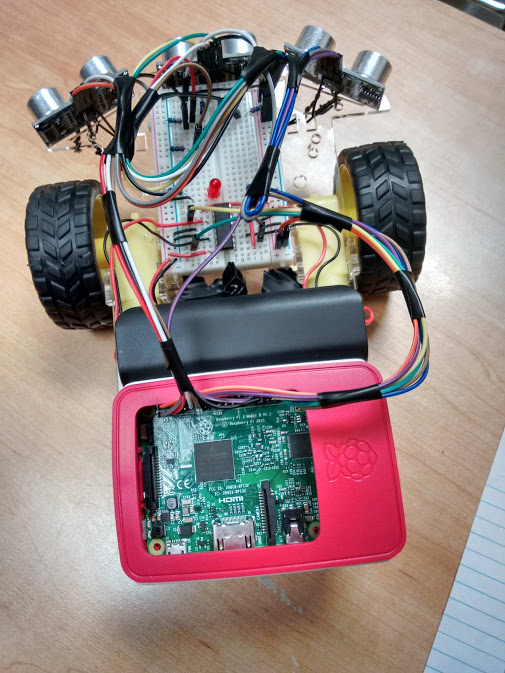
\includegraphics[width=\textwidth]{images/robot-top}
   \end{columns}
\end{frame}

\begin{frame}
   \frametitle{Four Major Principles of Object Oriented Programming}
   \begin{description}
   \item[Encapsulation]<2-> {\em Attributes} and {\em state} are contained 
     within objects and access to these attributes are restricted.
   \item[Abstraction]<3-> The inner workings of the objects are hidden.
   \item[Inheritance]<4-> Objects types can be derived from, and extend,
     other object types.  (Is-A relationship)
   \item[Polymorphism]<5-> Objects can be referenced by different types, 
     and they still behave correctly when treated as inherited types.
   \end{description}
\end{frame}

\begin{frame}
   \frametitle{Goals for Effective Object Oriented Programming}
   \begin{itemize}
   \item<2-> Your programs should be clear in intention.
   \item<3-> Objects should be cohesive.
   \item<4-> Objects should not be tightly coupled with other objects.
   \end{itemize}
\end{frame}

\section{Object Oriented Programming in C++}
\begin{frame}[fragile]
   \frametitle{Class Declaration}
   \begin{verbatim}
class name 
{
public:
    //public methods
protected:
    //protected variables and methods
private:
    //private variables and methods
}; 
   \end{verbatim}
\end{frame}

\begin{frame}
   \frametitle{Access Modifiers}
   \begin{description}
     \item[public] Accessible to code inside and outside of the class.
       \begin{itemize}
       \item<2-> Methods
       \item<2-> Constructors
       \item<2-> Destructor
       \end{itemize}
     \item[protected] Accessible to code within the class and sub-classes.
        (A big part of inheritance.)
        \begin{itemize}
        \item<3-> Variables (with great care)
        \item<3-> Methods
        \end{itemize}
     \item[private] Accessible only to code within the class.
         \begin{itemize}
         \item<4-> Variables
         \item<4-> Methods
         \end{itemize}
   \end{description}
\end{frame}

\begin{frame}[fragile]
   \frametitle{Constructors and Destructors}
   {\bf Constructors}
   \begin{itemize}
     \item Initializer for a class
     \item Can be overloaded
     \item Declared with same name as an object:
       {\tt name();}
     \item No return type
   \end{itemize}
   
   {\bf Destructor}
   \begin{itemize}
     \item Cleans up after an object.
     \item Used frequently with dynamic memory. 
     \item Named: {\tt $\sim$name();}
   \end{itemize}
\end{frame}

\begin{frame}[fragile]
   \frametitle{Member Initialization Lists}
   Member initialization lists can be used when simply copying values
   from constructor arguments.  They are an absolute must when working
   with references!
   \begin{verbatim}
name(int x, int y) : x(x), y(y)
{
  //constructor code
}
   \end{verbatim}
\end{frame}

\begin{frame}
   \frametitle{Constructor and Destructors Best Practices}
   \begin{itemize}
   \item Unless you really know what you are doing, constructors 
     should be public.
   \item You should provide at least:
   \begin{itemize}
     \item 1 No-Argument constructor: {\tt name(); }
     \item A copy constructor: {\tt name(name \&c); }
     \item If initial conditions make sense, you should have a constructor
       which allows them to be set.
   \end{itemize}
   \item If you use any dynamic memory, you must create a destructor.
   \end{itemize}
\end{frame}

\begin{frame}
   \frametitle{Putting it All Together}
   \begin{columns}
   \column{0.5\textwidth}
   Let's implement our robot class!
   
   \column{0.4\textwidth}
   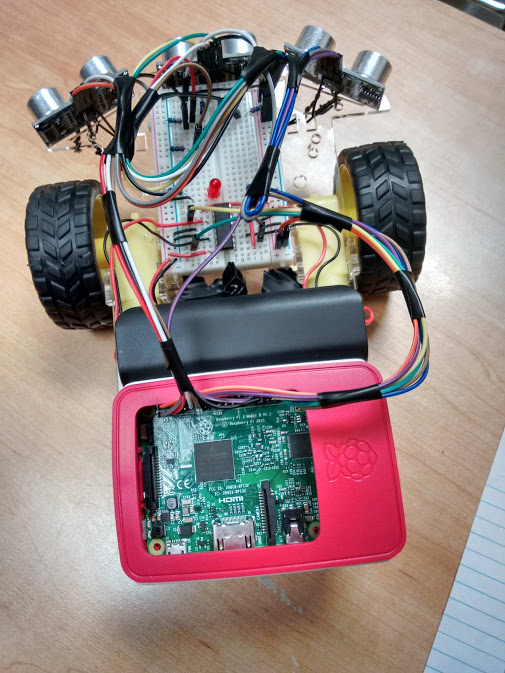
\includegraphics[width=\textwidth]{images/robot-top}
   \end{columns}
\end{frame}

\end{document}


